\documentclass[border=0pt]{standalone}
\usepackage{graphicx}
\usepackage{fancyvrb}
\usepackage{xcolor}
\usepackage{bm}
\usepackage{pgf}
\usepackage{tikz}


\definecolor{myGray}{rgb}{0.85,0.85,0.85}

\begin{document}

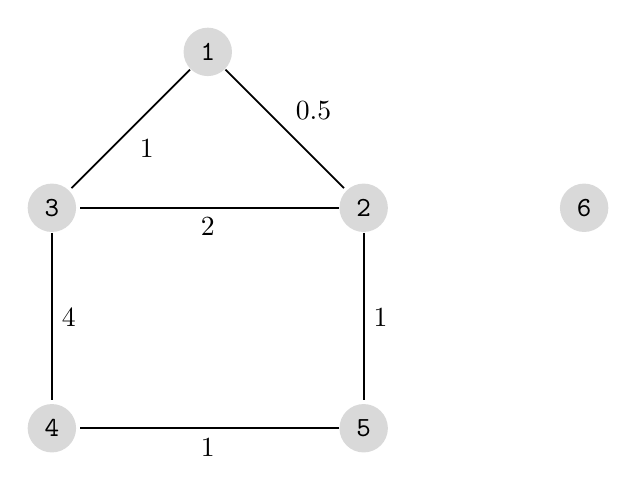
\begin{tikzpicture}[-,>=stealth,shorten >=1pt,auto,node distance=2.8cm,semithick]
  \tikzstyle{state}=[circle,fill=myGray,draw=none]

  \node[state] (1)                    {\texttt{1}};
  \node[state] (2) [below right of=1] {\texttt{2}};
  \node[state] (3) [below left of=1]  {\texttt{3}};
  \node[state] (4) [below of=3]       {\texttt{4}};
  \node[state] (5) [below of=2]       {\texttt{5}};
  \node[state] (6) [right of=2]       {\texttt{6}};

  \path (1) edge node {0.5} (2);
  \path (2) edge node {1}   (5);
  \path (5) edge node {1}   (4);
  \path (3) edge node {4}   (4);
  \path (1) edge node {1}   (3);
  \path (2) edge node {2}   (3);
\end{tikzpicture}

\end{document}
